\documentclass[10pt]{article}
\usepackage{amsmath, amssymb, enumitem, fancyhdr, graphicx, libertine, nth,
  pgfplots, tikz, xcolor}
\pgfplotsset{compat=1.11}
\usepackage[margin=1in]{geometry}
\usepackage[libertine]{newtxmath}
\pagestyle{fancy}
\definecolor{solution-color}{HTML}{000080}
\chead{\emph{EC201 -- Midterm Solutions}}

% Define new topic command
\newcommand{\topic}[1]{\medskip\begin{center}\large\textsc{#1}\normalsize
  \end{center}}

% Define question counter:
\newcounter{question}[section]
\newcommand{\question}[1]{\refstepcounter{question}
  \subsubsection*{Question~\thequestion~-- #1}}

% Subquestions are enumerate with letters
\newenvironment{subquestions}{
  \begin{enumerate}[label=(\roman*)]}{\end{enumerate}}

\begin{document}
\topic{Short Questions}
\question{Preferences (5 Points)}
The following are common assumptions about preferences:
\begin{itemize}
  \item Completeness
  \item Transitivity
  \item Monotonicity
  \item Convexity
\end{itemize}
Consider the following scenario:
\begin{itemize}
  \item I ask you which of the bundles $\left( x_1,x_2 \right)=\left( 2,2
    \right)$ and $\left(x_1,x_2  \right)=\left( 1, 5 \right)$ you prefer and you
    tell me you strictly prefer $\left( x_1,x_2 \right)=\left( 2,2 \right)$.
  \item I ask you which of the bundles $\left( x_1,x_2 \right)=\left( 1,5
    \right)$ and $\left( x_1,x_2 \right)=\left( 5,1 \right)$ you prefer and you
    tell me that you strictly prefer $\left( x_1,x_2 \right)=\left( 1,5
    \right)$.
  \item I ask you which of the bundles $\left( x_1,x_2 \right)=\left( 5,1
    \right)$ and $\left( x_1,x_2 \right)=\left( 2,2 \right)$ you prefer and you
    tell me that you strictly prefer $\left( x_1,x_2 \right)=\left( 5,1
    \right)$.
\end{itemize}
Which one of the common assumptions listed above do your choices violate and why?
\textcolor{solution-color}{
  From your choices we can gather the following:
  \begin{itemize}
    \item $\left( 2,2 \right)\succ \left( 1,5 \right)$
    \item $\left(1,5 \right)\succ\left( 5,1 \right)$
    \item $\left( 5,1 \right)\succ \left( 2,2 \right)$
  \end{itemize}
  Transitivity in short says that if $A\succ B$ and $B\succ C$, then it must be
  the case that $A\succ C$. Here it means that
  if you prefer $\left( 2,2 \right)$ to $\left( 1,5
  \right)$ and $\left( 1,5 \right)$ to $\left( 5,1 \right)$, then it must be
  the case that you prefer $\left( 2,2 \right)$ to $\left( 5,1 \right)$.
  However in the 3rd choice scenario, you chose $\left( 5,1 \right)$ over
  $\left( 2,2 \right)$, violating transitivity.
}

\textcolor{solution-color}{
  This doesn't violate completeness because you have a preference. This doesn't violate monotonicity because in no case did a bundle have at least as much of both goods with strictly more of one good. It doesn't violate convexity because one bundle cannot be written as a convex combination (a weighted average) of the other bundles.
}


\question{Technology (5 Points)}
The graph below shows an isoquant for a production function $f\left( x_1,x_2
\right)$.
\begin{center}
  \begin{tikzpicture}[baseline, scale = 0.5]
    \begin{axis}[xmax=6,xmin=0,
                 ymin=0,ymax=6,
                 domain=0.01:5.5,
                 xlabel=$x_1$,ylabel=$x_2$,
                 width=13cm]
      \addplot[samples=100] {2^(3/2) / x^(0.5)};
      \addplot[red, thick, samples=100, domain=0.1:0.7] {6.9 - 6 * x};
      \draw (0.4, 4.5) node {\Large{\textbullet}};
      \draw (0.4, 4.5) node [above right] {\Large{$A$}};
      \addplot[red, thick, samples=100, domain=2.4:5.5] {2.10 - 0.177 * x};
      \draw (4, 1.365) node {\Large{\textbullet}};
      \draw (4, 1.365) node [above right] {\Large{$B$}};
    \end{axis}
  \end{tikzpicture}
\end{center}
What do the slopes of the tangents at points $A$ and $B$ represent? How do we
interpret it?

\textcolor{solution-color}{
  The slopes of the tangent of an isoquant represents the technical rate of substitution ($TRS$). If we reduce $x_1$ a marginal amount, it measures how much extra $x_2$ we need to keep output constant. You could also have said that the move from $A$ to $B$ represents the diminishing rate of technical substitution.
}

\textcolor{solution-color}{
  \emph{For a longer answer (not required to get full points):}
}
\textcolor{solution-color}{
  The magnitude of the slope at $A$ is larger than at $B$ for the following
  reason. At $A$ we are currently using a lot of $x_2$ and not very much $x_1$.
  Since both $x_1$ and $x_2$ are needed for production (this is a convex
  production technology), if we reduce $x_1$ even further we need a large
  amount of $x_2$ to compensate us in order to be able to produce the same amount
  of output. At point $B$ we are using a lot of $x_1$ and not so much $x_2$. If
  we reduce $x_1$ a small amount we do not need to be compensated with very
  much $x_2$ in order to be able to produce the same amount of output.
}

\topic{Long Questions}

\question{Choice (15 Points)}
Your utility function for goods 1 and 2 is:
\[
  u\left( x_1,x_2 \right) = x_1^{\frac{2}{3}}x_2^{\frac{1}{3}}
\]
The prices of goods 1 and 2 are $p_1=2$ and $p_2=1$ respectively. You have $m=30$
income to spend.
\begin{subquestions}
  \item \textbf{[5 Points]} Find the marginal utility for goods 1 and 2,
    $MU_1$ and $MU_2$.
    \textcolor{solution-color}{
      \[
        MU_1 = \frac{\partial u\left( x_1,x_2 \right)}{\partial x_1}
        =\frac{2}{3}x_1^{\frac{2}{3}-1}x_2^{\frac{1}{3}}=
        \frac{2}{3}x_1^{-\frac{1}{3}}x_2^{\frac{1}{3}}
      \]
      \[
        MU_2 = \frac{\partial u\left( x_1,x_2 \right)}{\partial x_2}
        =\frac{1}{3}x_1^{\frac{2}{3}}x_2^{\frac{1}{3}-1}=
        \frac{1}{3}x_1^{\frac{2}{3}}x_2^{-\frac{2}{3}}
      \]
    }

  \item \textbf{[5 Points]} Find the marginal rate of substitution, $MRS$.
    \textcolor{solution-color}{
      \[
      MRS=- \frac{MU_1}{MU_2} =
      -\frac{\frac{2}{3}x_1^{\frac{2}{3}-1}x_2^{\frac{1}{3}}}
      {\frac{1}{3}x_1^{\frac{2}{3}}x_2^{-\frac{2}{3}}}=
      -2\frac{x_1^{-1}}{x_2^{-1}} = -\frac{2x_2}{x_1}
    \]
    }

  \item \textbf{[5 Points]} How much of goods 1 and 2 will you demand? Do not
    just write down the final answer. Derive the demand from the budget constraint
    and the consumer's optimality/tangency condition.
    \textcolor{solution-color}{
      The budget constraint is:
      \[
        p_1x_1+p_2x_2=m
      \]
      Using the values for $p_1$, $p_2$ and $m$:
      \[
        2x_1 + x_2 = 30
      \]
      The optimality condition is that we need to set
      $\left| MRS \right|=\frac{p_1}{p_2}$:
      \[
        \frac{2x_2}{x_1}=2
      \]
      This is just $x_1=x_2$. You will want to consume $x_1$ and $x_2$ in equal
      amounts. Using this in the budget constraint:
      \[
        2x_1 + x_2 = 30 \;\;\;\;\Longleftrightarrow \;\;\;\;
        2x_1 + x_1 = 30 \;\;\;\;\Longleftrightarrow \;\;\;\;
        3x_1 = 30 \;\;\;\;\Longleftrightarrow \;\;\;\; x_1 = 10
      \]
      And since $x_2=x_1$, $x_2 = 10$.
    }

\end{subquestions}

\question{Income and Substitution Effects (15 Points)}
There are two goods with prices $p_1$ and $p_2$. You have income $m$. According to your preferences for goods 1 and 2, good 1 is inferior (but not Giffen) and good 2 is a normal good. Your optimal bundle is a combination $\left( x_1,x_2 \right)$. If the price of good 1 falls from $p_1$ to $p_1^\prime$, you end up consuming \emph{more} of both goods 1 and 2, i.e.~your optimal bundle is $\left( x_1^\prime,x_2^\prime \right)$ where $x_1^\prime>x_1$ and $x_2^\prime>x_2$.
\begin{subquestions}
  \item \textbf{[5 Points]} Draw a graph showing the following:
    \begin{itemize}
      \item The budget constraints before the price of good 1 falls and after the price of good 1 falls. Label the vertical and horizontal intercepts.
      \item The optimal bundles before and after the price change, as well as the indifference curves associated with those optimal bundles.
    \end{itemize}
  \begin{tikzpicture}[scale=1]
    \draw [thick] (0,0) -- (8,0);
    \draw [thick] (0,0) -- (0,7);
    \node [right] at (8,0) {$x_1$};
    \node [above] at (0,7) {$x_2$};
    \draw [thick, blue] (0.2,5.1) to [out=310,in=160] (3.9,2.4);
    \draw [thick] (0.6,4) to [out=295,in=165] (3.5,1);
    \draw [thick, blue] (0,4.6) -- (7.5,0);
    \draw [thick] (0,4.6) -- (3.15,0);
    \draw[dotted](1.4,2.5)--(1.4,0);
    \draw[dotted](2.0,3.4)--(2.0,0);
    \node [left] at (1.3,2.5) {$x^A$};
    \draw[fill] (1.4,2.5) circle [radius =0.06];
    \node [right] at (2.0,3.6) {$x^C$};
    \draw[fill] (2.0,3.35) circle [radius =0.06];
    \node [left] at (0,4.6) {$\frac{m}{p_2}$};
    \node [below] at (3.15,0) {$\frac{m}{p_1}$};
    \node [below] at (7.5,0) {$\frac{m}{p_1^\prime}$};
  \end{tikzpicture}
  \item \textbf{[7 Points]} Draw a separate graph for this question. You will redraw your graph from part (i) but you will add the following:
    \begin{itemize}
      \item Show the income and substitution effect decomposition, i.e.~show the budget line that brings you back to your original purchasing power but with the new relative prices, the optimal bundle that you would choose on this budget line, and the indifference curve associated with that bundle. Identify where the income effect is and where the substitution effect is. \textbf{Remember, good 1 is an \emph{inferior} good}.
    \end{itemize}
  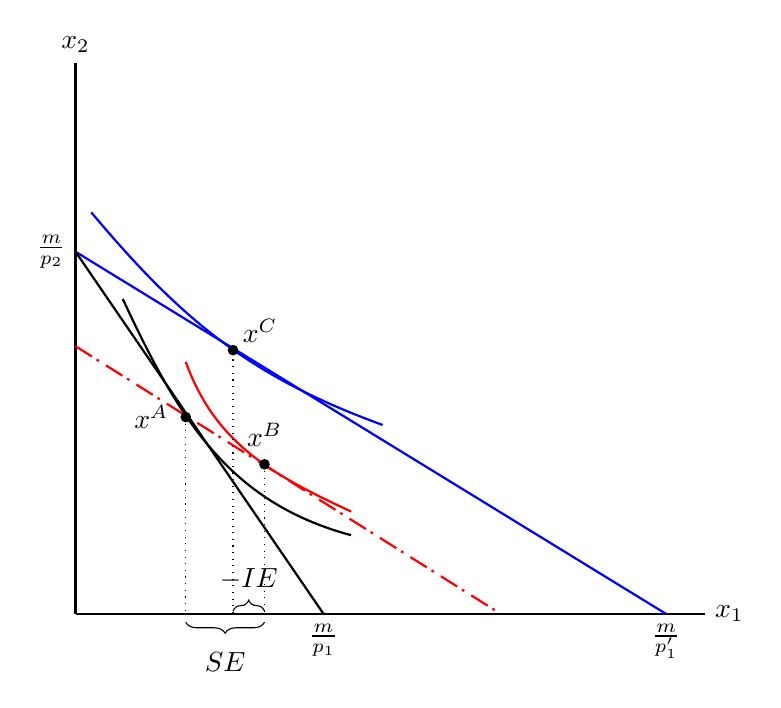
\begin{tikzpicture}[scale=1]
    \draw [thick] (0,0) -- (8,0);
    \draw [thick] (0,0) -- (0,7);
    \node [right] at (8,0) {$x_1$};
    \node [above] at (0,7) {$x_2$};
    \draw [thick, blue] (0.2,5.1) to [out=310,in=160] (3.9,2.4);
    \draw [thick] (0.6,4) to [out=295,in=165] (3.5,1);
    \draw [thick, red] (1.4,3.2) to [out=290,in=155] (3.5,1.3);
    \draw [thick, blue] (0,4.6) -- (7.5,0);
    \draw [thick] (0,4.6) -- (3.15,0);
    \draw[dotted](1.4,2.5)--(1.4,0);
    \draw[dotted](2.0,3.4)--(2.0,0);
    \draw [red,thick,dash pattern={on 7pt off 2pt on 1pt off 3pt}] (0,3.4) -- (5.4,0);
    \draw[dotted](2.4,1.9)--(2.4,0);
    \node [above] at (2.4,2) {$x^B$};
    \draw[fill] (2.4,1.9) circle [radius =0.06];
    \node [left] at (1.3,2.5) {$x^A$};
    \draw[fill] (1.4,2.5) circle [radius =0.06];
    \node [right] at (2.0,3.6) {$x^C$};
    \draw[fill] (2.0,3.35) circle [radius =0.06];
    \node [left] at (0,4.6) {$\frac{m}{p_2}$};
    \node [below] at (3.15,0) {$\frac{m}{p_1}$};
    \node [below] at (7.5,0) {$\frac{m}{p_1^\prime}$};
    \draw [decorate,decoration={brace,amplitude=4pt, mirror},xshift=0pt,yshift=-3pt]
    (1.4,0) -- (2.4,0) node [black,midway,yshift=-.5cm] {$SE$};
    \draw [decorate,decoration={brace,amplitude=4pt, mirror},xshift=0pt,yshift=1pt]
    (2.4,0) -- (2.0,0) node [black,midway,yshift=.4cm] {$-IE$};
  \end{tikzpicture}
  \item \textbf{[3 Points]} Compare the relative magnitudes of the income and substitution effect.

    \textcolor{solution-color}{
      The substitution effect is positive and the income effect is negative. However, the magnitude of the substitution effect is larger than the income effect.
    }
\end{subquestions}

% \question{Demand (15 Points)}
% Your demand functions for goods 1 and 2 are:
% \begin{align*}
%   x_1\left( p_1,p_2,m\right)&=\frac{2m - 100}{p_1} \\
%   x_2\left( p_1,p_2,m\right)&=\frac{100 - m}{p_2}
% \end{align*}
% % \begin{align*}
% %   x_1\left( p_1,p_2,m\right)&=
% %   \begin{cases}
% %     \frac{2m - 100}{p_1} &\text{ if } m \geq 50 \\
% %     0 & \text{ if } m < 50 \\
% %   \end{cases} \\
% %   x_2\left( p_1,p_2,m\right)&=
% %   \begin{cases}
% %     \frac{100 - m}{p_2} & \text{ if } m \leq 100 \\
% %     0 & \text{ if } m > 100 \\
% %   \end{cases}
% % \end{align*}
% Assume that $50\leq m\leq 100$ (this is not required to answer the question,
% but rather it is a a technical condition so that your demand for both goods is
% never negative).
% \begin{subquestions}
%   \item \textbf{[3 Points]} Is good 1 an ordinary or a Giffen good?
%   \item \textbf{[3 Points]} Is good 2 an ordinary or a Giffen good?
%   \item \textbf{[3 Points]} Is good 1 a normal good or an inferior good?
%   \item \textbf{[3 Points]} Is good 2 a normal good or an inferior good?
%   \item \textbf{[3 Points]} Is good 1 a substitute, a complement, or neither, for good 2?
% \end{subquestions}
\question{Intertemporal Choice (15 Points)}
\emph{In this question, please draw \textbf{separate} graphs for each part (i), (ii)
and (iii).}

\medskip\noindent
There are two periods. You receive income $m$ in period 1 and $m$ in period 2 (you receive the same amount of money in both periods, so in total you get $2m$ in your lifetime). You are able to borrow and lend at an interest rate $r$. There is no inflation.
\begin{subquestions}
  \item \textbf{[5 Points]} Draw the budget constraint. Label the axis
 intercepts and the endowment.

    \textcolor{solution-color}{
      \begin{tikzpicture}[scale=0.6]
        \draw[thick,<->] (0,11) node[above]{$c_2$}--(0,0)--(11,0)
          node[right]{$c_1$};
        \node [below left] at (0,0) {$0$};
        \node at (5,5) {\textbullet};
        \node [below left] at (5,5) {$\left( m,m \right)$};
        \draw(0,10)--(10,0);
        \node at (7, 3) [right] {$c_2 = m +\left( 1+r \right)\left(
        m-c_1 \right)$};
        \node at (0, 10) [left] {$m +\left( 1+r \right)m$};
        \node at (10, 0) [below] {$m +\frac{m}{1+r}$};
    \end{tikzpicture}
    }
\end{subquestions}
Your preferences, $u\left( c_1,c_2 \right)$, endowment, $\left( m_1,m_2 \right)$, and the interest rate, $r$, lead to you optimally choose a consumption path $\left( c_1,c_2 \right)$ where you \textbf{borrow} in the first period. That is, $c_1>m$.
\begin{subquestions}
  \setcounter{enumi}{1}
  \item \textbf{[5 Points]} Draw your optimal choice on a graph. Show the
    budget constraint, endowment, the optimal choice, and the indifference
    curve associated with the optimal choice.

    \textcolor{solution-color}{
      The optimal choice is where the indifference curve is tangent to the budget
      constraint. You borow in the first period so the optimal choice is
      \emph{south-east} of the endowment:
    }

    \textcolor{solution-color}{
      \begin{tikzpicture}[scale=0.6]
        \draw[thick,<->] (0,11) node[above]{$c_2$}--(0,0)--(11,0)
          node[right]{$c_1$};
        \node [below left] at (0,0) {$0$};
        \node [below] at (7,0) {$c_1^\star$};
        \node [left] at (0,3) {$c_2^\star$};
        \node at (7,3) {\textbullet};
        \node at (5,5) {\textbullet};
        \node [below left] at (5,5) {$\left( m,m \right)$};
        \draw (0,10)--(10,0);
        \draw [dotted] (0,3)--(7,3)--(7,0);
        \draw (4,8) ..controls (5.33,4) and (8,1.33) .. (11,1)
        node[right]{$u(c_1,c_2)=u^\star$};
    \end{tikzpicture}
    }

\end{subquestions}
Now the interest rate $r$, increases.
\begin{subquestions}
  \setcounter{enumi}{2}
  \item \textbf{[5 Points]} Show the change in the budget constraint on a graph. Can you still aford your original bundle?

    \textcolor{solution-color}{
      With an interest rate increase, the budget line pivots around the endownment.
    }

    \textcolor{solution-color}{
      \begin{tikzpicture}[scale=0.6]
        \draw[thick,<->] (0,13) node[above]{$c_2$}--(0,0)--(13,0)
          node[right]{$c_1$};
        \node [below left] at (0,0) {$0$};
        \node [below] at (7,0) {$c_1^\star$};
        \node [left] at (0,3) {$c_2^\star$};
        \node at (7,3) {\textbullet};
        \node at (5,5) {\textbullet};
        \node [below left] at (5,5) {$\left( m,m \right)$};
        \draw (0,10)--(10,0);
        \draw [red] (0,11)--(9.1,0);
        \draw [dotted] (0,3)--(7,3)--(7,0);
        \draw (4,8) ..controls (5.33,4) and (8,1.33) .. (11,1)
        node[right]{$u(c_1,c_2)=u^\star$};
    \end{tikzpicture}
    }

    \textcolor{solution-color}{
      You can no longer afford your optimal bundle from before.
    }
\end{subquestions}

\question{Uncertainty (15 Points)}
You have \$20,000 in your bank account. Your car is worth \$10,000 (so
altogether your wealth is \$30,000).  The probablity that your car will be
stolen in a given year is 10\%. An insurance company offers to insure your car
against theft for \$1,050 per year.  Your utility for wealth is $U\left( W
\right)=\sqrt{W}$.
\begin{subquestions}
  \item \textbf{[2 Points]} Are you risk averse, risk loving or risk neutral? Explain why.

    \textcolor{solution-color}{
      Your utility function is concave so you are risk averse.
    }

  \item \textbf{[4 Points]} What is your expected utility from \emph{not}
      purchasing insurance?

      \textcolor{solution-color}{
      If you do not purchase insurance, in the good state you keep your money
      in your bank account and your car. So you get \$30,000. In the bad state,
      your car is stolen and you only keep the money in your bank account. So
      you get \$20,000.  Therefore your expected utility is:
      \[
        0.9 \sqrt{30000} + 0.1 \sqrt{20000}=170.0267
      \]
    }

  \item \textbf{[4 Points]} What is your expected utility from purchasing
    insurance?

    \textcolor{solution-color}{
      If you purchase insurance, you get \$30,000-\$1,100=\$18,900 in both
      states. You get \$28,900 for certain. Your expected utility is then:
      \[
        \sqrt{28950}=170.147
      \]
    }

  \item \textbf{[2 Points]} Will you purchase insurance?

    \textcolor{solution-color}{
      Your expected utility from purchasing insurance is higher than if you
      didn't so you will purchase insurance.
    }

  \item \textbf{[3 Points]} How much would the actuarially fair insurance
    policy cost?

    \textcolor{solution-color}{
      The actuarially fair insurance costs what the expected value of the
      damage is.  Here it is $0.1 \times \$10,000 = \$ 1,000$.
    }

\end{subquestions}


\question{Cost curves, Firm Supply and Industry Supply (15 Points)}
There are 100 firms in a particular perfectly competitive industry. Each firm
has the following cost function:
\[
  c\left( y \right) = 2y^2 + 4
\]
The equilibrium price of output is $p$.
\begin{subquestions}
  \item \textbf{[2 Points]} What is the variable cost function $c_v\left( y
    \right)$?

    \textcolor{solution-color}{
    The variable cost function is $c_v\left( y \right)=2y^2$.
  }

  \item \textbf{[2 Points]}  What is the firm's fixed cost?

  \textcolor{solution-color}{
    The fixed cost is 4, the constant term in the cost function.
  }

  \item \textbf{[3 Points]}  What is the average cost function, $AC\left( y
    \right)$?

    \textcolor{solution-color}{
    \[
      AC\left( y \right)=\frac{c\left( y \right)}{y} = \frac{2y^2+4}{y} = 2y +
      \frac{4}{y}
    \]
  }

  \item \textbf{[3 Points]}  What is the marginal cost function, $MC\left( y
    \right)$?

    \textcolor{solution-color}{
    \[
      MC\left( y \right)=\frac{dc\left( y \right)}{dy}=4y
    \]
  }

  \item \textbf{[3 Points]}  What is firm $i$'s supply function, $S_i\left( p
    \right)$ (the supply function for one individual firm)?

  \textcolor{solution-color}{
    The firm will set $p=MC\left( y \right)$. So:
    \[
      p=4y \;\;\; \Longleftrightarrow \;\;\; y=\frac{4}{p}
      \;\;\; \Longleftrightarrow \;\;\; S_i\left( p
      \right)=\frac{p}{4}
    \]
  }

  \item \textbf{[2 Points]}  What is the industry supply function, $S\left( p
    \right)$?

  \textcolor{solution-color}{
    The industry supply function adds up all the individual supply functions:
    \[
      S\left( p \right)=S_1\left( p \right)+S_2\left( p
      \right)+\dots+S_{100}\left( p \right)=\frac{p}{4} +
      \frac{p}{4}+\dots+\frac{p}{4} = 100 \times \frac{p}{4}=\frac{25}{p}
    \]
  }
\end{subquestions}

\question{Equilibrium and Taxes (15 Points)}
The demand and supply functions for a particular good
  in the market are given by:
\[
  D\left( p \right) = 24 - 4p
\]
\[
  S\left( p \right) = 4 + 6p
\]
\begin{subquestions}
  \item \textbf{[6 Points]} Find the equilibrium price and quantity.

    \textcolor{solution-color}{
      To find the equilibrium price, $p^\star$, we set $D\left( p^\star
      \right)=S\left( p^\star \right)$:
    \[
      24-4p^\star=4+6p^\star \;\;\; \Longleftrightarrow \;\;\;
      24-4=4p^\star+6p^\star \;\;\; \Longleftrightarrow \;\;\;
      20=10p^\star \;\;\; \Longleftrightarrow \;\;\;
      p^\star=\frac{20}{10} \;\;\; \Longleftrightarrow \;\;\;
      p^\star=2
    \]
    The quantity can be found by using $p^\star$ in either $S\left( p
    \right)$ or $D\left( p \right)$. Using demand:
    \[
      q^\star = 24 - 4\times 2=16
    \]
    Using supply:
    \[
      q^\star = 4 + 6\times 2=16
    \]
    }


\end{subquestions}
Now the government imposes a per-unit tax (a quantity tax) of 1 on the good.
\begin{subquestions}
  \setcounter{enumi}{1}
  \item \textbf{[6 Points]}  Find the price the buyers pay, the price sellers
    receive and the new equilibrium quantity.

    \textcolor{solution-color}{
      Now $P_D=P_S+1$. We can replace $p$ in the demand function with $P_S+1$
      and then set demand equal to supply:
      \begin{align*}
        24 - 4\left( P_S+1 \right) &= 4+ 6P_S \\
        24 - 4P_S -4 &= 4 + 6P_S \\
        16  &=  10P_S \\
        P_S &= 1.6
      \end{align*}
      Using $P_D=P_S+1$ we can find the price buyers pay:
      \[
        P_D=1.6+1 = 2.6
      \]
      The price increased for buyers by 60 cents and the price
      decreased for sellers by 40 cents.
    }

    \textcolor{solution-color}{
      The new equilibrium quantity can be found using either the inverse demand
      or supply function. Using demand:
      \[
        q^\star = 24 - 4P_D = 2t - 4 \times 2.6 = 24 - 10.4 = 13.6
      \]
      Using supply:
      \[
        q^\star = 4 + 6P_S = 4 + 6 \times 1.6 = 4 + 9.6 = 13.6
      \]
      The tax decreased the equilibrium quantity by 2.4 units.
    }

  \item \textbf{[3 Points]}  What portion of the tax do consumers pay and what
    portion of the tax do sellers pay?

    \textcolor{solution-color}{
      Since the price increased by $\frac{3}{5}$ of the tax for consumers, they
      pay 60\% of the tax. The price decreased by $\frac{2}{5}$ of the tax for
      sellers so they pay 40\% of the tax.
    }
\end{subquestions}


\end{document}
